\chapter{Stable Neo-Hookean Flesh Simulation} \label{c:Paper}
In this chapter, I will examine further the topic of the paper \textit{\acrshort{snh}}, in particular, the calculations and conclusions made by the authors. I will go through each step they did, and my goal is to fill in some gaps to help in understanding the thought process. For this, I will include some of their calculations in more detail and add additional explanations. I would like to note that the information provided in this chapter is taken from the paper \acrshort{snh} if not stated otherwise. For simplification, I will not include a reference in each paragraph. 

The structure of this chapter is similar to the one of the paper: At first, I will go through the process of the formulation of the Stable Neo-Hookean energy. This includes pointing out the requirements and looking at existing energies. Finally, I will show that a complete eigenanalysis can be performed on the constructed energy.

\section{Deformation Gradient}
In the following, I will use the definitions involving the deformation gradient $\mathbf{F}$ introduced in \autoref{c:Background}. These definitions are summarized in Table \ref{table:gradient_quantities} for a better overview.

\setlength{\tabcolsep}{0.5em} % for the horizontal padding
{\renewcommand{\arraystretch}{1.1}% for the vertical padding
\begin{table}[!htbp]
\centering
    \begin{tabular}{ | l | l |}
    \hline
    \textbf{Symbol} & \textbf{Definition} \\ \hline
    $\mathbf{F} = \mathbf{RS}$ & Polar decomposition \\ \hline
    $J=\operatorname{det}(\mathbf{F})$ & Relative volume change \\ \hline
    $\mathbf{C}=\mathbf{F}^\mathsf{T} \mathbf{F}$ & Right Cauchy-Green tensor  \\ \hline	
    $I_{C}=\operatorname{tr}(\mathbf{C})$ & First right Cauchy-Green invariant \\ \hline
    \end{tabular}
    \caption[Quantities derived from the Deformation Gradient]{Quantities derived from the deformation gradient}
\label{table:gradient_quantities}
\end{table}

\newpage
\section{Energy Formulation}
In this section, I will go through the process of formulating a new deformation energy. At first, I will explain what properties a deformation energy should have. Secondly, I will analyse existing energies. Finally, I will go through the formulation of the novel energy from the paper \acrshort{snh}.

\subsection{Stability} 
\label{ss:stability}
The core goal of the paper was to model deformations for virtual characters that have human-like features. In order to achieve better results than what has been done in current research, they formulated a new deformation energy. In \autoref{c:Background}, I concluded that the appropriate energy for animating soft tissues such as flesh has to be hyperelastic. Another important property is the stability of the energy. We need a hyperelastic energy that is stable in the following four ways, which were introduced in the paper itself:

\textbf{1. Inversion Stability:} Given some arbitrary object, it is possible that while deforming the object, we can arrive at a zero volume state or even an entire inversion. For example, we can look at the tetrahedron shown in Fig. \ref{fig:inversion_1}. In Fig. \ref{fig:inversion_2}, we see a deformed state of this tetrahedron where the volume is scaled down to zero, and we are left with a simple triangle. In Fig. \ref{fig:inversion_3}, the tetrahedron arrives at an inverted state. The deformation energy has to be able to deal with both cases without creating severe artefacts. That means that the energy has to be singularity-free, meaning that it is defined for every possible point. This property should ideally hold without needing any filters or threshold.
\begin{figure}[!ht]
\centering
\begin{subfigure}{.3\textwidth}
  \centering
  % include first image
  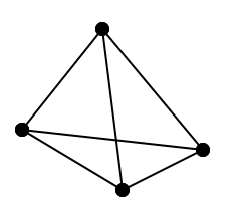
\includegraphics[width=.8\linewidth]{resources/stability_inversion_1.png}  
  \caption{Rest state}
  \label{fig:inversion_1}
\end{subfigure}
\begin{subfigure}{.3\textwidth}
  \centering
  % include first image
  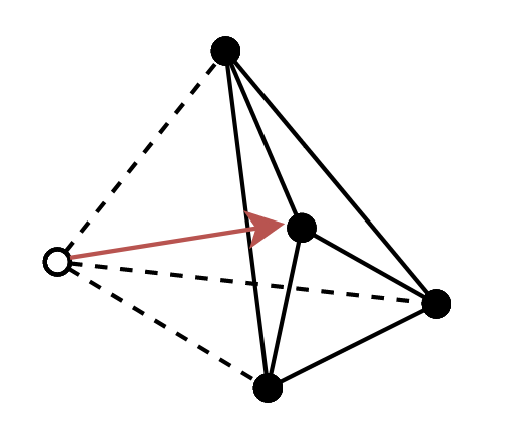
\includegraphics[width=.9\linewidth]{resources/stability_inversion_2.png}  
  \caption{Zero-volume state}
  \label{fig:inversion_2}
\end{subfigure}
\begin{subfigure}{.3\textwidth}
  \centering
  % include second image
  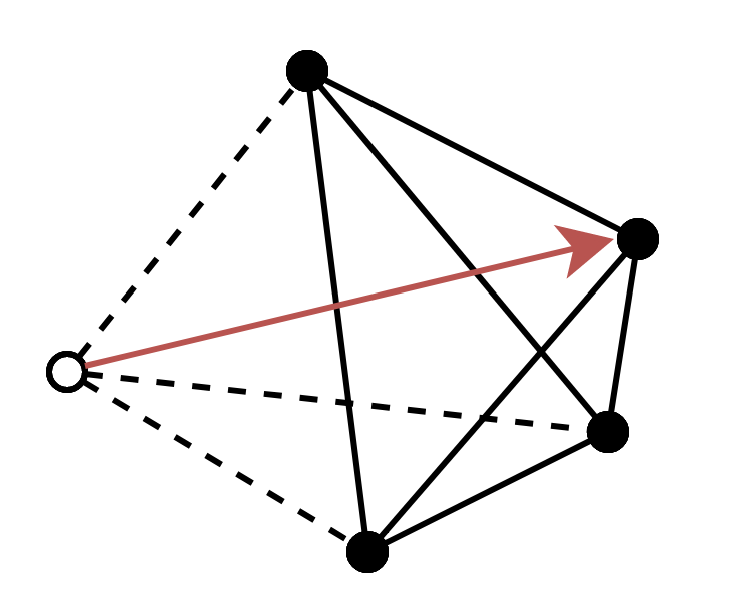
\includegraphics[width=.9\linewidth]{resources/stability_inversion_3.png}  
  \caption{Inverted state}
  \label{fig:inversion_3}
\end{subfigure}
\caption[Inversion of a tetrahedron]{Inversion of a tetrahedron}
\label{fig:inversion}
\end{figure}

\textbf{2. Reflection stability:} While deforming an object, it can occur that we are dealing with reflections. An example of a reflection in 2D is shown in Fig. \ref{fig:reflection}. The coloured triangle is reflected over the y-axis. A matrix that represents a reflection is orthogonal with a determinant equal to $-1$. The deformation energy needs to be well behaved under reflections. This has to hold, regardless of the reflection convention used in the \acrshort{svd} of \textbf{F}. The reflection convention is explained in \autoref{c:Background} in \autoref{ss:svd_deformation_gradient}.
\begin{figure}[!htbp]
	\centering
	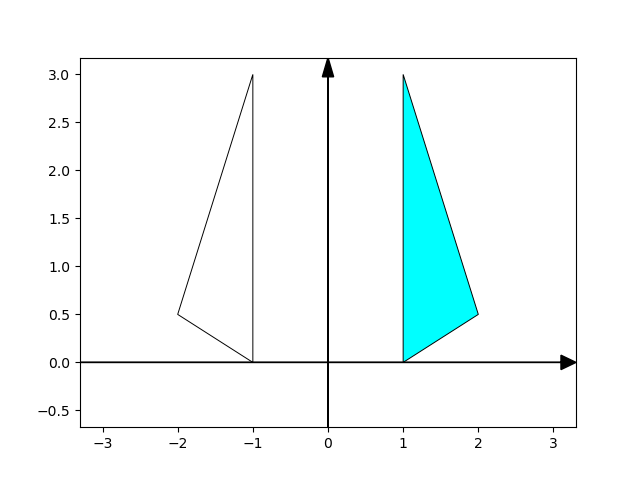
\includegraphics[width=0.5\textwidth]{resources/reflection_plot.png}
	\caption[Reflection of a triangle over the y-axis]{Reflection of a triangle over the y-axis}
	\label{fig:reflection}
\end{figure}

\textbf{3. Rest stability:} While deforming an object in a certain way, we apply one or multiple forces to that object, which influences the deformation. But if we remove all the forces, the object should be able to go back into its rest state. This ability was introduced in \autoref{c:Background} as elasticity.

\textbf{4. Meta-stability under degeneracy:} Here we are dealing with a special case of deformation. If we crush a volumetric object into a plane, line, or point, we change the object into a degenerate case. This process is illustrated for a cube in Fig. \ref{fig:meta_stability}. Even with these extreme conditions, the object should still be able to recover into its actual shape and not some other.
\begin{figure}[!htbp]
	\centering
	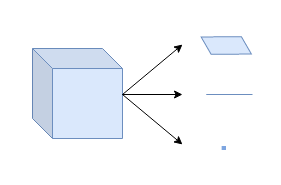
\includegraphics[width=0.5\textwidth]{resources/metastability.png}
	\caption[Illustration of meta stability]{Illustration of degeneracy}
	\label{fig:meta_stability}
\end{figure}

Based on these four requirements, I will judge the existing models for the deformation energy. These criteria determine whether a proposed energy is suited for simulating the fleshy look or not.

\subsection{Existing Neo-Hookean Energies}
In previous literature, a few energies were proposed, which I will analyse in this section. They are listed in Table \ref{table:energies}. All of these energies were formulated for hyperelastic materials.

\setlength{\tabcolsep}{0.5em} % for the horizontal padding
{\renewcommand{\arraystretch}{1.3}% for the vertical padding
\begin{table}[!htbp]
\centering
    \begin{tabular}{ | l | l |}
    \hline
    \textbf{Energy} & \textbf{Author(s)} \\ \hline
    $\Psi_{Neo}=\frac{\mu}{2}\left(I_{C}-3\right)-\mu \log J+\frac{\lambda}{2}(\log J)^{2}$ & \begin{tabular}{@{}l@{}}e.g. Bonet and Wood 1997 \\ (\cite{bonet1997nonlinear})\end{tabular}  \\ \hline
    $\Psi_{\mathrm{A}}=\frac{\mu}{2}\left(I_{C}-3\right)-\mu \log J+\frac{\lambda}{2}(J-1)^{2}$ & Odgen 1997 (\cite{ogden1997non}) \\ \hline
    $\Psi_{\mathrm{B}}=\frac{\mu}{2}\left(J^{-2 / 3} I_{C}-3\right)+\frac{\lambda}{2}(J-1)^{2}$ & Bower 2009 (\cite{bower2009applied}) \\ \hline
    $\Psi_{\mathrm{C}}=\frac{\mu}{2}\left(J^{-2 / 3} I_{C}-3\right)+\frac{\lambda}{2}(J-1)$ & \begin{tabular}{@{}l@{}}Wang and Yang 2016 \\ (\cite{wang2016descent}) \end{tabular} \\ \hline
    \end{tabular}
    \caption[Summary of proposed energies]{Summary of proposed energies (\cite{Smith:2018:SNF:3191713.3180491})}
\label{table:energies}
\end{table}

According to the Valanis-Landel hypothesis, many hyperelastic energies can be split up into a 1D length, 2D area, and 3D volume term. The energies in Table \ref{table:energies} only contain the length and volume term. Hence, each of these energies can be separated into a 1D length term and a 3D volume term. The 1D length term penalizes the length changes an object undergoes during a deformation, whereas the 3D volume term penalizes the change in volume of the object.

\setlength{\tabcolsep}{0.5em} % for the horizontal padding
{\renewcommand{\arraystretch}{1.3}% for the vertical padding
\begin{table}[!htbp]
\centering
    \begin{tabular}{ | l | l | l |}
    \hline
    \textbf{Energy} & \textbf{1D length term} & \textbf{3D volume term} \\ \hline
    $\Psi_{Neo}$ & $\frac{\mu}{2}\left(I_{C}-3\right)$ & $-\mu \log J+\frac{\lambda}{2}(\log J)^{2}$ \\ \hline
    $\Psi_{\mathrm{A}}$ & $\frac{\mu}{2}\left(I_{C}-3\right)$ & $-\mu \log J+\frac{\lambda}{2}(J-1)^{2}$ \\ \hline
    $\Psi_{\mathrm{B}}$ & $\frac{\mu}{2}\left(J^{-2 / 3} I_{C}-3\right)$ & $\frac{\lambda}{2}(J-1)^{2}$ \\ \hline
    $\Psi_{\mathrm{C}}$ & $\frac{\mu}{2}\left(J^{-2 / 3} I_{C}-3\right)$ & $\frac{\lambda}{2}(J-1)$ \\ \hline
    \end{tabular}
    \caption{Energies split up into their 1D length and 3D volume term}
\label{table:energies_split}
\end{table}

\subsubsection{1D Length Term}
The term that is used for $\Psi_{Neo}$ and $\Psi_{A}$ is defined as
\[
\Psi_{M}=\frac{\mu}{2}\left(I_{C}-3\right).
\]
This energy was originally proposed by Mooney in 1940 (\cite{mooney1940theory}). It is today known as the Neo-Hookean energy because of Rivlin (\cite{rivlin1948large}). If we expand the term with the singular values of the deformation gradient \textbf{F}, we get the following equation:
\[
\Psi_{M}=\frac{\mu}{2}\left(\sigma_{0}^2 + \sigma_{1}^2 + \sigma_{2}^2 - 3\right)
\]
The term reaches its minimum at a zero volume state, meaning at $I_{C}=0$, which leads to $\Psi_{M}=-3$. Because this is not desirable, Mooney added the hard constraint that $J$ should be equal to $1$. Hence, the energy is minimized at a volume-preserving configuration. Note that the energy is singularity free and well defined under inversion.

The second term is defined by
\[
\Psi_{R} = \frac{\mu}{2}\left(J^{-2 / 3} I_{C}-3\right).
\]
It is used in $\Psi_{B}$ and $\Psi_{C}$. This term was introduced by Rivlin in 1948 (\cite{rivlin1948large}). Using the singular values of \textbf{F}, we get the following expression:
\[
\Psi_{R} = \frac{\mu}{2}\left(\frac{\sigma_{0}^2 + \sigma_{1}^2 + \sigma_{2}^2}{(\sigma_{0}  \sigma_{1}  \sigma_{2})^\frac{2}{3}}
 - 3\right)
\]
Unfortunately, this term is not singularity free. If $J$ is equal to zero, the result is not defined anymore.

\subsubsection{3D Volume Term}
The volume term of $\Psi_{Neo}$ is described as
\[
\Psi_{Neo, volume} = -\mu \log J+\frac{\lambda}{2}(\log J)^{2}
\]
and results in numerical problems since the logarithmic function is not defined for $J<0$ and grows unbounded for $J \rightarrow 0$. In conclusion, $\Psi_{Neo, volume}$ is not singularity free. 
The same applies to the 3D volume term of $\Psi_{A}$, namely
\[
\Psi_{A, volume} = -\mu \log J+\frac{\lambda}{2}(J-1)^{2}.
\]
The volume term of $\Psi_{B}$ and $\Psi_{C}$ is of the form
\[
\Psi_{B, volume} = \frac{\lambda}{2}(J-1)^{2}
\]
and does not have these problems. It is bounded, well defined, and invertible. After these observations, the authors of \acrshort{snh} combined the robust length term with the robust volume term and received $\Psi_D$, which is defined as
\[
\Psi_{D} = \frac{\mu}{2}\left(I_{C}-3\right) +\frac{\lambda}{2}(J-1)^{2}.
\]
$\Psi_{D}$ is singularity free and well defined under inversion. Unfortunately, it does not satisfy the requirement of being rest stable, which I will discuss in the next section.

In addition, we can see that each of the proposed energies contains a term that is not well defined under certain conditions. That means that each of the energies in Table \ref{table:energies} is not singularity free or well defined under inversion and therefore confirms the need for the formulation of a new energy.

\subsection{Rest Stabilization}
Although $\Psi_{D}$ meets almost all stated requirements, it is not rest stable. We can show that with the \acrlong{pk1} (\acrshort{pk1}). For our case, it is defined as
\begin{equation}\label{eq:pk1}
P(\mathbf{F}) = \frac{\partial \Psi}{\partial \mathbf{F}} (\mathbf{F}).
\end{equation}
With the help of Eq. \eqref{eq:pk1} we can calculate the \acrshort{pk1} of $\Psi_{D}$. For the following calculations, keep in mind that $I_{C} = \operatorname{tr}(\mathbf{F}^\mathsf{T} \mathbf{F})$ and $J = \operatorname{det}(\mathbf{F})$ holds with $\mathbf{F}$ being the deformation gradient. I will use the explicit terms during the calculations for a better understanding.
\begin{align*}
P_{D}(\mathbf{F}) &= \frac{\partial \Psi_{D}}{\partial \mathbf{F}} (\mathbf{F}) = \frac{\partial}{\partial \mathbf{F}} \left[ \frac{\mu}{2}\left(I_{C}-3\right) +\frac{\lambda}{2}(J-1)^{2} \right] \\
&= \frac{\partial}{\partial \mathbf{F}} \left[ \frac{\mu}{2}\left(\operatorname{tr}(\mathbf{F}^\mathsf{T} \mathbf{F})-3\right) +\frac{\lambda}{2}(\operatorname{det}(\mathbf{F})-1)^{2} \right] \\
&= \frac{\partial}{\partial \mathbf{F}}  \frac{\mu}{2}\left(\operatorname{tr}(\mathbf{F}^\mathsf{T} \mathbf{F})-3\right) +\frac{\partial}{\partial \mathbf{F}} \frac{\lambda}{2}(\operatorname{det}(\mathbf{F})-1)^{2}
\end{align*}
Looking at the two terms separately, we get:
\begin{align*}
&\frac{\partial}{\partial \mathbf{F}} \frac{\mu}{2} (\operatorname{tr}(\mathbf{F}^\mathsf{T} \mathbf{F}) - 3) = \frac{\mu}{2} \, 2 \mathbf{F} = \mu \mathbf{F}
\\
&\frac{\partial}{\partial \mathbf{F}} \frac{\lambda}{2} (\operatorname{det}(\mathbf{F})-1)^{2} = \frac{\lambda}{2} \frac{\partial \operatorname{det}(\mathbf{F})}{\partial \mathbf{F}} \, 2 (\operatorname{det}(\mathbf{F}) - 1) = \lambda \frac{\partial \operatorname{det}(\mathbf{F})}{\partial \mathbf{F}}(\operatorname{det}(\mathbf{F})-1)
\end{align*}
Hence, $P_{D}$ resolves to
\[
P_{D}(\mathbf{F}) = \mu \mathbf{F} + \lambda \frac{\partial \operatorname{det}(\mathbf{F})}{\partial \mathbf{F}}(\operatorname{det}(\mathbf{F})-1).
\]
In order to find out whether an energy is rest stable or not, we can set the input variable to the identity matrix $\mathbf{I}$. An energy is rest stable if $P(\mathbf{I})=0$ (\cite{Smith:2018:SNF:3191713.3180491}). Unfortunately, this is not the case for $\Psi_{D}$:
\[
P_{D}(\mathbf{I}) = \mu \mathbf{I} + \lambda \frac{\partial \operatorname{det}(\mathbf{I})}{\partial \mathbf{F}}(\operatorname{det}(\mathbf{I})-1) = \mu \mathbf{I} \neq 0
\]
That is problematic because if we simulate a deformation, the object will shrink in volume when it should be back in its rest state. In order to solve this problem, the authors modified $(J-1)^{2}$ to $(J-\alpha)^{2}$. Using this modification, the energy shifts to
\[
\Psi_{E} = \frac{\mu}{2}\left(I_{C}-3\right) +\frac{\lambda}{2}(J-\alpha)^{2}.
\]
Now \acrshort{pk1} for $\Psi_E$ can be calculated similarly as before, and we get:
\begin{align*}
P_{E}(\mathbf{F}) &= \frac{\partial \Psi_{E}}{\partial \mathbf{F}} = \frac{\partial}{\partial \mathbf{F}}  \left[ \frac{\mu}{2}\left(I_{C}-3\right) +\frac{\lambda}{2}(J-\alpha)^{2} \right] \\
&= \frac{\partial}{\partial \mathbf{F}}  \left[ \frac{\mu}{2}\left(\operatorname{tr}(\mathbf{F}^\mathsf{T} \mathbf{F})-3\right) +\frac{\lambda}{2}(\operatorname{det}(\mathbf{F})-\alpha)^{2} \right] \\
&= \mu \mathbf{F} + \lambda \frac{\partial \operatorname{det}(\mathbf{F})}{\partial \mathbf{F}} (\operatorname{det}(\mathbf{F})-\alpha)
\end{align*}
Solving for an alpha that satisfies $P_{E}(\mathbf{I})=0$ gives us $\alpha=1+\frac{\mu}{\lambda}$. Now $\Psi_{E}$ has to be changed accordingly:
\[
\Psi_{E} = \frac{\mu}{2}\left(I_{C}-3\right) +\frac{\lambda}{2}(J-1-\frac{\mu}{\lambda})^{2}
\]
We can now expand the quadratic and obtain
\[
\Psi_{E} = \frac{\mu}{2}\left(I_{C}-3\right) - \mu\left(J-1\right) + \frac{\lambda}{2}(J-1)^{2} + \left(\frac{\mu}{\lambda}\right)^{2}.
\]
Since constants disappear under differentiation, this expression is functionally equivalent to 
\begin{equation}\label{energy_without_barrier}
\Psi_{E} = \frac{\mu}{2}\left(I_{C}-3\right) - \mu\left(J-1\right) + \frac{\lambda}{2}(J-1)^{2}.
\end{equation}
Note that $\Psi_{E}$ looks very similar to $\Psi_{Neo}$. The difference is that $log(J)$ is replaced with $(J-1)$ in $\Psi_{E}$. Keep in mind that $(J-1)$ is the first term of the Taylor approximation of $\operatorname{log}(J)$ at $J=1$:
\[
\operatorname{log}(J) = \boldsymbol{(J-1)} - \frac{1}{2} (J-1)^{2} + \frac{1}{3} (J-1)^{3} + \text{...}
\]
Thus, $\Psi_{E}$ can be looked at as an approximation of $\Psi_{Neo}$ that is singularity-free and has rest stability. In addition, it has reflection stability because $I_{C}$ contains the squared singular values of $\mathbf{F}$. Hence, any negation convention is irrelevant, and the $J$ term contains the product of the singular values, so the sign convention is again irrelevant. Therefore, $\Psi_{E}$ has inversion, reflection, and rest stability.

\subsection{Meta-Stability under Degeneracy}
We know from the last section that the energy $\Psi_{E}$ has inversion, reflection, and rest stability. Now we are interested in how it behaves under degeneracy. The authors of the paper \textit{\acrshort{snh}} viewed this examination as a Drucker stability analysis (see e.g. \cite{bower2009applied}). Drucker stability describes a set of criteria that a material can satisfy or not. It is a measurement of the stability of a material. The calculations can be found in the supplemental material of \textit{\acrshort{snh}}. I will only present the results here. 

The energy remains stable when crushing the object into a \textit{plane}. The object is able to return to its rest state. Thus, no further adjustments need to be done. When crushing the object into a \textit{line}, the energy is meta-stable. The object will self-restore into the correct shape after any perturbations. A possible perturbation could be a momentum. The alternative would be a state that yields singularities, which is not desirable. Hence, we can leave the energy as it is. We can also crush the object to a \textit{point}, which results in $\mathbf{F} = 0$. In this case, the material cannot recover into its rest state. This effect is small for a higher Poisson's ratio. For completeness, the authors nevertheless added a regularized origin barrier:
\[
	\Psi_{origin} = - \frac{\mu}{2}\operatorname{log}(I_C +\delta)
\]
This term eliminates the unwanted behaviour for point compression for all positive Poisson's ratio, without interfering with the other requirements for the energy. It can be shown that the value of $\delta$ should be set to $1$. This proof is also included in the supplemental material of the paper.

We can now write the final energy down as
\begin{equation}\label{eq:stable_energy}
\boxed{\Psi_{new} = \frac{\mu}{2}\left(I_{C}-3\right) + \frac{\lambda}{2}(J-\alpha)^{2} - \frac{\mu}{2} \operatorname{log}\left(I_{C}+1\right).}
\end{equation}
With this adjustment the rest stability term shifts to $\alpha=1+\frac{\mu}{\lambda}-\left(\frac{\mu}{4}\right)\lambda$.

To note here is that the authors mainly introduced this origin barrier because of pedagogical completeness. In practice, the origin barrier was not needed, and the version of the energy without it, formulated in Eq. \eqref{energy_without_barrier}, was used.

\subsection{Lamé Reparameterization}
Because of the origin barrier introduced in the last section, we need to make a reparametrization of the Lamé parameters $\lambda$ and $\mu$. As I explained in \autoref{ss:deformation_energy}, there is a non-linear relationship between the stresses and strains for hyperelastic materials for larger strain predictions. But for infinitesimal deformation, we should still be consistent with Hooke's law. In order to reach this goal, the model needs to reproduce the \acrshort{pk1} of linear elasticity, which is defined as
\begin{equation} \label{eq:reparametrization}
	\mathbf{P}(\mathbf{F}) = 2 \mu_{\text{\textit{Lamé}}} \epsilon + \lambda_{\text{\textit{Lamé}}} \operatorname{tr}(\epsilon) \mathbf{I},
\end{equation}
where $\epsilon = \frac{1}{2} (\mathbf{F} + \mathbf{F}^\mathsf{T}) - \mathbf{I}$ is the linearized strain tensor and $\mu_{\text{\textit{Lamé}}}$ and $\lambda_{\text{\textit{Lamé}}}$ are the Lamé parameters in linear elasticity. If we linearize the stress from Eq. \eqref{eq:stable_energy} and keep it consistent with the form described in Eq. \eqref{eq:reparametrization}, the values shift to $\mu = \frac{4}{3} \mu_{\text{\textit{Lamé}}}$ and $\lambda = \lambda_{\text{\textit{Lamé}}} + \frac{5}{6} \mu_{\text{\textit{Lamé}}}$. The equation for the Poisson's ratio then shifts to 
\[
	\nu = \frac{\lambda - \left( \frac{5}{8} \right) \mu}{2 \left(\lambda + \left( \frac{1}{8} \right) \mu  \right)}.
\]
These reparameterized expressions for the Lamé parameters were used in all of the tests made in the paper \acrshort{snh}. In addition, with these formulations, it can be shown that the energy does not introduce any spurious minima in the range of $\nu \in [0, 0.5)$. The details are again given in the supplemental material of the paper \acrshort{snh}.

\section{Energy Analysis}
In order to simulate physical deformations, we put some constraints on an object and minimize the deformation energy. Thus, we need a minimization tool. In this case, we will use Newton's method. I will further explain Newton's method in \autoref{s:optimization}. But first, we need to know more about the properties of the energy. The goal of this chapter is to show that a complete eigenanalysis can be performed on the new energy, formulated in Eq. \eqref{eq:stable_energy}, which will help us form a qualitative understanding of the energy.

\subsection{First Piola-Kirchhoff Stress (\acrshort{pk1})}
In order to analyse the energy and build the Hessian terms, the first step is to calculate \acrshort{pk1} for Eq. \eqref{eq:stable_energy} with $\alpha=1+\frac{\mu}{\lambda}-\left(\frac{\mu}{4}\right)\lambda$. Again, $I_{C}$ is equal to $\operatorname{tr}(\mathbf{F}^\mathsf{T} \mathbf{F})$, $J$ signifies $\operatorname{det}(\mathbf{F})$, and I am using the explicit terms during the calculations. With this, we can calculate $P_{new}$ by
\begin{align*}
P_{new}(\mathbf{F}) &= \frac{\partial \Psi_{new}}{\partial \mathbf{F}} = \frac{\partial}{\partial \mathbf{F}} \left[ \frac{\mu}{2}\left(I_{C}-3\right) + \frac{\lambda}{2}(J-\alpha)^{2} - \frac{\mu}{2}\operatorname{log}\left(I_{C}+1\right) \right]
\\
&= \frac{\partial}{\partial \mathbf{F}} \left[ \frac{\mu}{2}\left(\operatorname{tr}(\mathbf{F}^\mathsf{T} \mathbf{F})-3\right) + \frac{\lambda}{2}(\operatorname{det}(\mathbf{F})-\alpha)^{2} - \frac{\mu}{2}\operatorname{log}\left(\operatorname{tr}(\mathbf{F}^\mathsf{T} \mathbf{F})+1\right) \right] .
\end{align*}
Similar to before, I am looking at the terms separately:
\begin{align*}
&\frac{\partial}{\partial \mathbf{F}} \frac{\mu}{2}\left(\operatorname{tr}(\mathbf{F}^\mathsf{T} \mathbf{F})-3\right) = \mu \mathbf{F}
\\
&\frac{\partial}{\partial \mathbf{F}} \frac{\lambda}{2}(\operatorname{det}(\mathbf{F})-\alpha)^{2} = \lambda (\operatorname{det}(\mathbf{F})-\alpha)  \frac{\partial \operatorname{det}(\mathbf{F})}{\partial \mathbf{F}} 
\\ 
&\frac{\partial}{\partial \mathbf{F}} \frac{\mu}{2}\operatorname{log}\left(\operatorname{tr}(\mathbf{F}^\mathsf{T} \mathbf{F})+1\right) = \frac{\mu}{2} \, 2 \mathbf{F} \, \frac{1}{\operatorname{tr}(\mathbf{F}^\mathsf{T} \mathbf{F}) + 1} = \mu \mathbf{F} \frac{1}{\operatorname{tr}(\mathbf{F}^\mathsf{T} \mathbf{F}) + 1}
\end{align*}
When we combine these terms again, we get to the final formula of $P_{new}$:
\begin{align*}
P_{new}(\mathbf{F}) &= \mu \mathbf{F} + \lambda (\operatorname{det}(\mathbf{F})-\alpha)  \frac{\partial \operatorname{det}(\mathbf{F})}{\partial \mathbf{F}} - \mu \mathbf{F} \frac{1}{\operatorname{tr}(\mathbf{F}^\mathsf{T} \mathbf{F}) + 1} \\
&= \mu \left( 1 - \frac{1}{\operatorname{tr}(\mathbf{F}^\mathsf{T} \mathbf{F}) + 1}\right) \mathbf{F} + \lambda( \operatorname{det}(\mathbf{F})-\alpha)\frac{\partial  \operatorname{det}(\mathbf{F})}{\partial \mathbf{F}}
\end{align*}
By using $I_{C}$ and $J$, we get the following expression for $P_{new}(\mathbf{F})$:
\[
	P_{new}(\mathbf{F}) = \mu \left( 1 - \frac{1}{I_{C} + 1}\right) \mathbf{F} + \lambda( J-\alpha)\frac{\partial  J}{\partial \mathbf{F}}
\]
A convenient shorthand for computing $\frac{\partial J}{\partial \mathbf{F}}$ is to write the expression as a result of cross products:
\begin{equation}\label{eq:cross_product}
\frac{\partial J}{\partial \mathbf{F}} = \left[ \,\mathbf{f_1} \times \mathbf{f_2}\, \bigg| \,\mathbf{f_2} \times \mathbf{f_0}\, \bigg| \,\mathbf{f_0} \times \mathbf{f_1}\, \right],
\end{equation}
where $\mathbf{f_i}$ signify the column vectors of $\mathbf{F}$ defined in Eq. \eqref{eq:deformation_gradient}. This formulation is also handy when analysing $\frac{\partial^2 J}{\partial \mathbf{F}^2}$.

\subsection{The Energy Hessian Terms}
In the following, I will derive the Hessian terms of the energy. In addition, I will examine the eigenvalues and eigenvectors. This information about the Hessian is important for the optimization process because, with it, we can determine the definiteness of the matrix. 

The Hessian matrix will be a ($9 \times 9$)-matrix. It is demanding to keep an overview while working with high dimensional matrices. In order to not lose sight, we can write the Hessian of the energy as a fourth-order matrix-of-matrices by using the scalar notation for $\mathbf{F}$ defined in Eq. \eqref{eq:deformation_gradient}:
\[
\frac{\partial^2 \Psi_{new}}{\partial \mathbf{F}^2} = \frac{\partial P_{new}(\mathbf{F})}{\partial \mathbf{F}} = 
\left[\begin{array}{ccc}{\left[\frac{\partial P_{new}(\mathbf{F})}{\partial f_0}\right]} & {\left[\frac{\partial P_{new}(\mathbf{F})}{\partial f_3}\right]} & {\left[\frac{\partial P_{new}(\mathbf{F})}{\partial f_6}\right]} \\ {\left[\frac{\partial P_{new}(\mathbf{F})}{\partial f_1}\right]} & {\left[\frac{\partial P_{new}(\mathbf{F})}{\partial f_4}\right]} & {\left[\frac{\partial P_{new}(\mathbf{F})}{\partial f_7}\right]} \\ {\left[\frac{\partial P_{new}(\mathbf{F})}{\partial f_2}\right]} & {\left[\frac{\partial P_{new}(\mathbf{F})}{\partial f_5}\right]} & {\left[\frac{\partial P_{new}(\mathbf{F})}{\partial f_8}\right]} \end{array}\right]
\]
The advantage of this form is that we can look at each entry separately, which improves readability. Each entry of the Hessian is defined as
\begingroup
\addtolength{\jot}{0.8em}
\begin{align} \label{eq:final_entries_hessian}
	\frac{\partial P_{new}(\mathbf{F})}{\partial f_i} = \frac{\partial}{\partial f_i} \left[ \mu \left( 1 - \frac{1}{I_{C} + 1}\right) \mathbf{F} + \lambda(J-\alpha)\frac{\partial J}{\partial \mathbf{F}} \right] \nonumber
	\\
	\stackrel{\text{prod.rule}}{=} \underbrace{\frac{\partial \mathbf{F}}{\partial f_i} \mu \left( 1 - \frac{1}{I_{C} + 1}\right)}_{\mathbf{T}_{i}}  + \underbrace{\mu \frac{2}{\left(I_{C} + 1\right)^2} \mathbf{F} f_i}_{_{\mathbf{M}_{i}}}
	\\
	+ \underbrace{\lambda \frac{\partial J}{\partial \mathbf{F}} \frac{\partial J}{\partial f_i}}_{_{\mathbf{G}_{i}}}+ \underbrace{\lambda (J- \alpha) \frac{\partial^2 J}{\partial \mathbf{F}\partial f_i}}_{_{\mathbf{H}_{i}}}. \nonumber
\end{align}
\endgroup
This final equation looks quite complicated. But we can split it up into these four terms: A $\mathbf{T}_i$ (Tikhonov), $\mathbf{M}_i$ (Mu), $\mathbf{G}_i$ (volume Gradient), and a $\mathbf{H}_i$ (volume Hessian) term. In the following, I will examine each of these terms separately. This way, we do not have to deal with one large and complicated expression immediately.

\subsection{The Tikhonov, Mu, and Gradient Terms}
\subsubsection{Tikhonov}
The Tikhonov term from Eq. \eqref{eq:final_entries_hessian} is a ($9 \times 9$)-matrix and can be written in form of a fourth-order matrix-of-matrices. It is defined as
\[
	\frac{\partial \mathbf{F}}{\partial f_i} \mu \left( 1 - \frac{1}{I_{C} + 1}\right).
\]
With the explicit term for $I_{C}$, this expression resolves to
\[
	\frac{\partial \mathbf{F}}{\partial f_i} \mu \left( 1 - \frac{1}{\operatorname{tr}(\mathbf{F}^\mathsf{T} \mathbf{F}) + 1}\right).
\]
Explicitly computing the Tikhonov term is not very difficult. In order to compute this term, we need to calculate $\mathbb{T} = \frac{\partial \mathbf{F}}{\partial f_i}$. So, we have mainly entries of zeros except for the $i$-th entry. Therefore, $\mathbb{T}$ can be calculated by
\[
\mathbb{T} = \left[\begin{array}{ccc}{\begin{bmatrix} 1 & 0 & 0 \\ 0 & 0 & 0 \\ 0 & 0 & 0 \end{bmatrix}} & {\begin{bmatrix} 0 & 1 & 0 \\ 0 & 0 & 0 \\ 0 & 0 & 0 \end{bmatrix}} & {\begin{bmatrix} 0 & 0 & 1 \\ 0 & 0 & 0 \\ 0 & 0 & 0 \end{bmatrix}} \\ {\begin{bmatrix} 0 & 0 & 0 \\ 1 & 0 & 0 \\ 0 & 0 & 0 \end{bmatrix}} & {\begin{bmatrix} 0 & 0 & 0 \\ 0 & 1 & 0 \\ 0 & 0 & 0 \end{bmatrix}} & {\begin{bmatrix} 0 & 0 & 0 \\ 0 & 0 & 1 \\ 0 & 0 & 0 \end{bmatrix}} \\ {\begin{bmatrix} 0 & 0 & 0 \\ 0 & 0 & 0 \\ 1 & 0 & 0 \end{bmatrix}} & {\begin{bmatrix} 0 & 0 & 0 \\ 0 & 0 & 0 \\ 0 & 1 & 0 \end{bmatrix}} & {\begin{bmatrix} 0 & 0 & 0 \\ 0 & 0 & 0 \\ 0 & 0 & 1 \end{bmatrix}} \end{array}\right].
\]
If we vectorize $\mathbb{T}$, we get the identity matrix $\mathbf{I} \in \mathbb{R}^{9x9}$, which is of full rank, positive definite, and independent of the values in \textbf{F}: 
\[
\operatorname{vec}(\mathbb{T}) =  \mathbf{\check{T}} = \mathbf{I} = \in \mathbb{R}^{9x9}
\]
In addition, the Tikhonov term serves as a diagonal regularizer for the rest of the energy.

\subsubsection{Mu}
The Mu term from Eq. \eqref{eq:final_entries_hessian} is again a ($9 \times 9$)-matrix and can be written in the form of a fourth-order matrix-of-matrices. It is described by the following expression:
\[
	\mu \frac{2}{\left(I_{C} + 1\right)^2} \mathbf{F} f_i
\]
With the explicit term for $I_{C}$, the Mu term resolves to
\[
	\mu \frac{2}{\left(\operatorname{tr}(\mathbf{F}^\mathsf{T} \mathbf{F} + 1\right)^2} \mathbf{F} f_i.
\]
In order to compute the Mu term, we need to calculate $\mathbb{M} = \mathbf{F} f_i$. That means that the $i$-entry is squared, and the remaining entries do not change. Therefore, $\mathbb{M}$ takes on the following form:
\[
\mathbb{M} = \left[\begin{array}{ccc}{\begin{bmatrix} f_0^2 & f_0f_3 & f_0f_6 \\ f_0f_1 & f_0f_4 & f_0f_7 \\ f_0f_2 & f_0f_5 & f_0f_8 \end{bmatrix}} & {\begin{bmatrix} f_3f_0 & f_3^2 & f_3f_6 \\ f_3f_1 & f_3f_4 & f_3f_7 \\ f_3f_2 & f_3f_5 & f_3f_8 \end{bmatrix}} & {\begin{bmatrix} f_6f_0 & f_6f_3 & f_6^2 \\ f_6f_1 & f_6f_4 & f_6f_7 \\ f_6f_2 & f_6f_5 & f_6f_8 \end{bmatrix}} \\ {\begin{bmatrix} f_1f_0 & f_1f_3 & f_1f_6 \\ f_1^2 & f_1f_4 & f_1f_7 \\ f_1f_2 & f_1f_5 & f_1f_8 \end{bmatrix}} & {\begin{bmatrix} f_4f_0 & f_4f_3 & f_4f_6 \\ f_4f_1 & f_4^2 & f_4f_7 \\ f_4f_2 & f_4f_5 & f_4f_8 \end{bmatrix}} & {\begin{bmatrix} f_7f_0 & f_7f_3 & f_7f_6 \\ f_7f_1 & f_7f_4 & f_7^2 \\ f_7f_2 & f_7f_5 & f_7f_8 \end{bmatrix}} \\ {\begin{bmatrix} f_2f_0 & f_2f_3 & f_2f_6 \\ f_2f_1 & f_2f_4 & f_2f_7 \\ f_2^2 & f_2f_5 & f_2f_8 \end{bmatrix}} & {\begin{bmatrix} f_5f_0 & f_5f_3 & f_5f_6 \\ f_5f_1 & f_5f_4 & f_5f_7 \\ f_5f_2 & f_5^2 & f_5f_8 \end{bmatrix}} & {\begin{bmatrix} f_8f_0 & f_8f_3 & f_8f_6 \\ f_8f_1 & f_8f_4 & f_8f_7 \\ f_8f_2 & f_8f_5 & f_8^2 \end{bmatrix}} \end{array}\right]
\]
Again, $f_i$ stand for the scalar entries of $\mathbf{F}$. When vectorizing $\mathbb{M}$, the diagonal of the resulting matrix $\mathbf{\check{M}}$ consists of the squared values of $f_i$:
\[
\operatorname{vec}(\mathbb{M})= \mathbf{\check{M}} = \begin{bmatrix} f_0^2 & f_1f_0 & f_2f_0 & f_3f_0 & f_4f_0 & f_5f_0 & f_6f_0 & f_7f_0 & f_8f_0 \\ f_0f_1 & f_1^2 & f_2f_1 & f_3f_1 & f_4f_1 & f_5f_1 & f_6f_1 & f_7f_1 & f_8f_1 \\ f_0f_2 & f_1f_2 & f_2^2 & f_3f_2 & f_4f_2 & f_5f_2 & f_6f_2 & f_7f_2 & f_8f_2 \\ f_0f_3 & f_1f_3 & f_2f_3 & f_3^2 & f_4f_3 & f_5f_3 & f_6f_3 & f_7f_3 & f_8f_3 \\ f_0f_4 & f_1f_4 & f_2f_4 & f_3f_4 & f_4^2 & f_5f_4 & f_6f_4 & f_7f_4 & f_8f_4 \\ f_0f_5 & f_1f_5 & f_2f_5 & f_3f_5 & f_4f_5 & f_5^2 & f_6f_5 & f_7f_5 & f_8f_5 \\ f_0f_6 & f_1f_6 & f_2f_6 & f_3f_6 & f_4f_6 & f_5f_6 & f_6^2 & f_7f_6 & f_8f_6 \\ f_0f_7 & f_1f_7 & f_2f_7 & f_3f_7 & f_4f_7 & f_5f_7 & f_6f_7 & f_7^2 & f_8f_7 \\ f_0f_8 & f_1f_8 & f_2f_8 & f_3f_8 & f_4f_8 & f_5f_8 & f_6f_8 & f_7f_8 & f_8^2 \end{bmatrix}
\]
This structure makes it possible to express $\mathbf{\check{M}}$ more conveniently. We can write $\mathbf{\check{M}}$ as an outer product of $\operatorname{vec}(\mathbf{F}) = \mathbf{\check{f}}$:
\[
\mathbf{\check{M}}= \operatorname{vec}(\mathbf{F})\operatorname{vec}(\mathbf{F})^\mathsf{T} = \mathbf{\check{f}} \mathbf{\check{f}}^\mathsf{T}
\]
This matrix is of rank one and has a single non-zero eigenvalue. In order to examine the eigenvalues, we can calculate
\[
\| \mathbf{\check{f}} \|^{2}_{2} = \sum_{n=0}^8 | f_n |^2 = \| \mathbf{F} \|^{2}_{F} = \sum_{n=0}^3 \sigma^2_i = \left( \sigma_0^2 + \sigma_1^2 + \sigma_2^2 \right),
\]
in which $\|\cdot\|_F$ stands for the Frobenius norm introduced in Def. \ref{FN}, and $\sigma_i$ are the singular values from $\mathbf{\Sigma}$ in the \acrshort{svd} of $\mathbf{F}$ stated in Eq. \eqref{eq:svd_simga}. This expression can be obtained by using Eq. \eqref{eq:FN}. The eigenvector of $\mathbf{\check{M}}$ is $\mathbf{\check{f}} / \| \mathbf{\check{f}} \|$. The eigenvalue is always non-negative and large if $\mathbf{F}$ contains a large stretch.

\subsubsection{Volume Gradient}
The volume Gradient term from Eq. \eqref{eq:final_entries_hessian} is also a ($9 \times 9$)-matrix and can be written in the form of a fourth-order matrix-of-matrices. The Gradient term is defined as
\[
	\lambda \frac{\partial J}{\partial \mathbf{F}} \frac{\partial J}{\partial f_i},
\]
with $J=\operatorname{det}(\mathbf{F})$. Since $\lambda$ is just a scalar constant, we are more interested in the term 
\[
\mathbb{G} = \frac{\partial J}{\partial \mathbf{F}} \frac{\partial J}{\partial fi}.
\]
As already mentioned, we can write $\partial J / \partial \mathbf{F}$ in the form of cross products (see Eq. \eqref{eq:cross_product}) to make its computation easier. We can then set $\operatorname{vec}(\partial J / \partial \mathbf{F}) = \mathbf{\check{g}}$ and write the vectorized matrix $\mathbf{\check{G}}$ as an outer product of $\mathbf{\check{g}}$:
\[
\operatorname{vec}(\mathbb{G})) = \mathbf{\check{G}} = \operatorname{vec}\left(\frac{\partial J}{\partial \mathbf{F}}\right) \operatorname{vec}\left(\frac{\partial J}{\partial \mathbf{F}}\right)^\mathsf{T} = \mathbf{\check{g}} \mathbf{\check{g}}^\mathsf{T}
\]
There is again a single non-zero, non-negative eigenvalue. We can calculate it by
\[
\| \mathbf{\check{g}} \|^2_2 = \left\| \frac{\partial J}{\partial \mathbf{F}} \right \|^2_F = \left[ (\sigma_0 \sigma_1)^2 + (\sigma_0 \sigma_2)^2 + (\sigma_1 \sigma_2)^2 \right].
\]
The corresponding eigenvector is $\mathbf{\check{g}} / \| \mathbf{\check{g}} \|$.

\subsection{The Volume Hessian}
\label{ss:volume_hessian}
The volume Hessian term from Eq. \eqref{eq:final_entries_hessian} is again a ($9 \times 9$)-matrix. But this time, the computation is a bit trickier. The term is described by
\[
	\lambda (J- \alpha) \frac{\partial^2 J}{\partial \mathbf{F}\partial f_i}
\]
with $J=\operatorname{det}(\mathbf{F})$. The term that needs special attention is the following:
\[
\mathbb{H} = \frac{\partial^2 J}{\partial \mathbf{F} \partial f_i}
\]
We can write this term again in the form of a fourth-order matrix-of-matrices:
\[
\mathbb{H} = \frac{\partial^2 J}{\partial \mathbf{F} \partial f_i} = \left[\begin{array}{ccc}{\frac{\partial}{\partial \mathbf{F}}\left[\frac{\partial J}{\partial f_0}\right]} & {\frac{\partial}{\partial \mathbf{F}}\left[\frac{\partial J}{\partial f_3}\right]} & {\frac{\partial}{\partial \mathbf{F}}\left[\frac{\partial J}{\partial f_6}\right]} \\ {\frac{\partial}{\partial \mathbf{F}}\left[\frac{\partial J}{\partial f_1}\right]} & {\frac{\partial}{\partial \mathbf{F}}\left[\frac{\partial J}{\partial f_4}\right]} & {\frac{\partial}{\partial \mathbf{F}}\left[\frac{\partial J}{\partial f_7}\right]} \\ {\frac{\partial}{\partial \mathbf{F}}\left[\frac{\partial J}{\partial f_2}\right]} & {\frac{\partial}{\partial \mathbf{F}}\left[\frac{\partial J}{\partial f_5}\right]} & {\frac{\partial}{\partial \mathbf{F}}\left[\frac{\partial J}{\partial f_8}\right]} \end{array}\right]
\]
The entries of $\mathbb{H}$ have a specific form. For example, the first entry resolves to
\begin{align*}
	\frac{\partial}{\partial \mathbf{F}}\left[\frac{\partial J}{\partial f_0}\right] &= \frac{\partial}{\partial \mathbf{F}} \frac{\partial}{\partial f_0} \left[ f_0 f_4 f_8 + f_2 f_3 f_7 + f_1 f_5 f_6 - f_2 f_4 f_6 - f_0 f_5 f_7 - f_1 f_3 f_8 \right]
	\\ 
	&= \frac{\partial}{\partial \mathbf{F}} \left[ f_4 f_8 - f_5 f_7 \right] = 
	\left[ \begin{matrix}
0 & 0 & 0 \\ 0 & f_8 & -f_5 \\ 0 & -f_7 & f_4 \end{matrix} \right].
\end{align*}
Vectorizing this matrix reveals the vector $\left[ 0,\, 0,\, 0,\, 0,\, f_8,-f_7,\,0,-f_5,\,f_4 \right]^\mathsf{T}$. 

By repeating this procedure, $\mathbf{\check{H}}$ reveals the structure
\[
\operatorname{vec}(\mathbb{H}) = \mathbf{\check{H}} = \begin{bmatrix} 0 & 0 & 0 & 0 & f_8 & -f_7 & 0 & -f_5 & f_4 \\ 0 & 0 & 0 & -f_8 & 0 & f_6 & f_5 & 0 & -f_3 \\ 0 & 0 & 0 & f_7 & -f_6 & 0 & -f_4 & f_3 & 0 \\ 0 & -f_8 & f_7 & 0 & 0 & 0 & 0 & f_2 & -f_1 \\ f_8 & 0 & -f_6 & 0 & 0 & 0 & -f_2 & 0 & f_0 \\ -f_7 & f_6 & 0 & 0 & 0 & 0 & f_1 & -f_0 & 0 \\ 0 & f_5 & -f_4 & 0 & -f_2 & f_1 & 0 & 0 & 0 \\ -f_5 & 0 & f_3 & f_2 & 0 & -f_0 & 0 & 0 & 0 \\ f_4 & -f_3 & 0 & -f_1 & f_0 & 0 & 0 & 0 & 0 \end{bmatrix}.
\]
When we look at the matrix, we can see a pattern for the entries. $\mathbf{\check{H}}$ is of the form:
\[
\mathbf{\check{H}} = \left[ \begin{matrix}
0 & -\mathbf{\widehat{F_2}} & \mathbf{\widehat{F_1}} \\ \mathbf{\widehat{F_2}} & 0 & -\mathbf{\widehat{F_0}} \\ -\mathbf{\widehat{F_1}} & \mathbf{\widehat{F_0}} & 0 \end{matrix} \right].
\]
Matrices that have this structure are called cross-product matrices. By looking at the entries separately, we can observe that they reveal the same structure. So, each $\mathbf{\widehat{F_i}}$ is also a cross-product matrix. This property is called \textit{self-similarity}. Therefore, $\mathbf{\check{H}}$ is a \textit{self-similar} cross-product matrix. 

\subsubsection{Volume Hessian Eigenvalues}
In the following, I will determine the eigenvalues of $\mathbf{\check{H}}$. In order to calculate the eigenvalues of a matrix, we need the corresponding characteristic polynomial. The characteristic polynomial of a square matrix $\mathbf{A}$ is defined by
\[
	p(\epsilon) = \operatorname{det}(\mathbf{A}-\epsilon \, \mathbf{I}),
\]
where $\epsilon$ symbolizes the eigenvalues of $\mathbf{A}$. The eigenvalues can be calculated by setting $p(\epsilon)$ to zero (\cite{Spencer1980}, p. 27-28). Because $\mathbf{\check{H}}$ is a ($9 \times 9$)-matrix, we expect it to have nine eigenvalues: $\epsilon_0$, $\epsilon_2$, ..., $\epsilon_8$. In order to determine the eigenvalues, we can factor $\mathbf{\check{H}}$ into the following two characteristic polynomials:
\begin{align}
p_1(\epsilon) &= \epsilon^3 - \operatorname{tr}(\mathbf{C}) \epsilon - 2 J  \label{vol_hessian_eq1} \\
p_2(\epsilon)&=\epsilon^3 - \operatorname{tr}(\mathbf{C}) \epsilon^2 + \frac{1}{2} \left( \operatorname{tr^2}(\mathbf{C}) - \operatorname{tr}(\mathbf{C}^2) \right) \epsilon - \operatorname{det}(\mathbf{C}) \label{vol_hessian_eq2}
\end{align}
First, I examine $p_2(\epsilon)$ from Eq. \eqref{vol_hessian_eq2}. It is easier to solve because it corresponds to the characteristic polynomial of $\mathbf{C}$. Given its roots $\epsilon_\alpha$, $\epsilon_\beta$, $\epsilon_\gamma$, we can calculate six of the eigenvalues of $\mathbf{\check{H}}$, namely $\pm \sqrt{\epsilon_\alpha}$, $\pm \sqrt{\epsilon_\beta}$, $\pm \sqrt{\epsilon_\gamma}$. Using the singular values of $\mathbf{F}$, these eigenvalues can be written in the following form:
\begin{align}
\label{eq:hessian_eigenvalues1}
\epsilon_3 &= \sqrt{\epsilon_\alpha} = \sigma_0 & \epsilon_6 &= -\sqrt{\epsilon_\alpha} = -\sigma_0 \nonumber \\
\epsilon_4 &=  \sqrt{\epsilon_\beta} = \sigma_1 & \epsilon_7 &=  -\sqrt{\epsilon_\beta} = -\sigma_1 \\
\epsilon_5 &= \sqrt{\epsilon_\gamma} = \sigma_2 & \epsilon_8 &= -\sqrt{\epsilon_\gamma} = -\sigma_2 \nonumber
\end{align}
The remaining eigenvalues can be obtained by using $p_1(\epsilon)$ from Eq. \eqref{vol_hessian_eq1}. This equation represents a depressed cube. A depressed cube is a cubic that can be expressed by
\[
t^3 + q_1t + q_2. 
\]
$p_1(\epsilon)$ can be written in this form with $q_1=-\operatorname{tr}(\mathbf{C})$ and $q_2= -2J$. Using this knowledge, the roots of $p_1(\epsilon)$ and therefore the remaining eigenvalues $\epsilon_0$, $\epsilon_1$, $\epsilon_2$ of $\mathbf{\check{H}}$ can be obtained by
\begin{equation}
\label{eq:hessian_eigenvalues2}
	\epsilon_k = 2 \sqrt{\frac{I_C}{3}} \operatorname{cos}\left[ \frac{1}{3} \left( \operatorname{arccos}\left(\frac{3 J}{I_C} \sqrt{\frac{3}{I_C}} \right) + 2 \pi k \right) \right] \quad  k= 0,1,2.
\end{equation}
These are all eigenvalues of $\mathbf{\check{H}}$. Three of the six eigenvalues ($\epsilon_3$, ..., $\epsilon_8$) have to be negative or equal to zero since the root function yields a positive and a negative value. In addition, the cosine function for calculating $\epsilon_0$, $\epsilon_1$, and $\epsilon_2$ ensures that one or two of these eigenvalues are also negative. 

We have now found the eigenvalues of the terms of $\frac{\partial^2 \Psi_{new}}{\partial \mathbf{F}^2}$, described in Eq. \eqref{eq:final_entries_hessian}. We found out that except for the volume Hessian term, all terms only have non-negative eigenvalues. Thus, the volume Hessian is the only source of negative eigenvalues.

In order to investigate the behaviour of the volume Hessian term further, we need to look at $J = \operatorname{det}(\mathbf{F})$ a bit more in detail. $J$ is not convex, which is problematic for the optimization process. Fortunately, the other terms of $\frac{\partial^2 \Psi_{new}}{\partial \mathbf{F}^2}$ serve as an additional regularization, as already stated for the Tikhonov term.

\subsubsection{Volume Hessian Eigenvectors}
In this section, I will show the eigenvectors of $\mathbf{\check{H}}$. According to the eigendecomposition, $\mathbf{\check{H}}$ can be factorized as $\mathbf{\check{H}} = \mathbf{\check{Q}}\mathbf{\Lambda}\mathbf{\check{Q}}^\mathsf{T}$. We can obtain the eigenvectors by computing $\mathbf{\check{Q}}$. To be consistent with the procedure so far, I will use the tensor form symbolized by $\mathbb{Q}$:
\[
\mathbb{Q} = \left[\begin{array}{ccc}{\left[\mathbf{Q}_0\right]} & {\left[\mathbf{Q}_3\right]} & {\left[\mathbf{Q}_6\right]} \\ {\left[\mathbf{Q}_1\right]} & {\left[\mathbf{Q}_4\right]} & {\left[\mathbf{Q}_7\right]} \\ {\left[\mathbf{Q}_2\right]} & {\left[\mathbf{Q}_5\right]} & {\left[\mathbf{Q}_8\right]} \end{array}\right]
\]
Each entry of $\mathbf{\check{Q}}$ is an eigenvector in the form of a ($3 \times 3$)-matrix instead of a vector with nine entries. I am starting with the eigenvalues obtained by Eq. \eqref{vol_hessian_eq2}, namely $\epsilon_3$, $\epsilon_4$, ..., $\epsilon_8$. The eigenvectors corresponding to these eigenvalues can all be written in the following form:
\begin{equation}\label{eq:eigenvectors_vhessian}
\mathbf{Q}_k = \frac{1}{\sqrt{2}} \mathbf{U} \mathbf{D}_k \mathbf{V}^\mathsf{T} \qquad \qquad \text{for } k = 3, 4, ..., 8
\end{equation}
\textbf{U} and \textbf{V} are taken from the \acrshort{svd} of \textbf{F}, and $\frac{1}{\sqrt{2}}$ is a normalization factor. The difference of the eigenvectors lies in the matrix $\mathbf{D}_k$. For each eigenvalue $\epsilon_k$ for $k \in {3,4,...,8}$, $\mathbf{D}_k$ is defined as:
\begin{align*}
&\mathbf{D_3} = \left[ \begin{matrix}
0 & 0 & 0 \\ 0 & 0 & 1 \\ 0 & -1 & 0 \end{matrix} \right] &\mathbf{D}_6 = \left[ \begin{matrix}
0 & 0 & 0 \\ 0 & 0 & 1 \\ 0 & 1 & 0 \end{matrix} \right]
 \\[0.5em]
&\mathbf{D_4} = \left[ \begin{matrix}
0 & 0 & 1 \\ 0 & 0 & 0 \\ -1 & 0 & 0 \end{matrix} \right] &\mathbf{D}_7 = \left[ \begin{matrix}
0 & 0 & 1 \\ 0 & 0 & 0 \\ 1 & 0 & 0 \end{matrix} \right]
 \\[0.5em]
&\mathbf{D_5} = \left[ \begin{matrix}
0 & 1 & 0 \\ -1 & 0 & 0 \\ 0 & 0 & 0 \end{matrix} \right] &\mathbf{D}_8 = \left[ \begin{matrix}
0 & 1 & 0 \\ 1 & 0 & 0 \\ 0 & 0 & 0 \end{matrix} \right]
\end{align*}
These eigenvectors have a unique \textit{pseudo-cross-product} structure. $\mathbf{D_3}$ is a cross-product matrix for the basis vector $[-1, 0, 0]^\mathsf{T}$. In addition, $\mathbf{Q}_6$ differs from $\mathbf{Q}_3$ only because of one sign. Therefore, $\mathbf{D}_3$ has been multiplied by a reflection, which makes $\mathbf{Q}_6$ a reflected pseudo-cross-product matrix. $\mathbf{Q}_4$ and $\mathbf{Q}_5$ are in the same way cross-product matrices for the basis vectors $[0, -1, 0]^\mathsf{T}$ and $[0, 0, -1]^\mathsf{T}$. $\mathbf{Q}_7$ and $\mathbf{Q}_8$ are the corresponding reflected pseudo-cross-product matrices.

The remaining eigenvectors correspond to the eigenvalues $\epsilon_0$, $\epsilon_1$, and $\epsilon_2$ derived from the depressed cubic. They are of the form
\[
\mathbf{Q}_k = \frac{1}{\| \mathbf{D}_k \|_{F}} \mathbf{U} \mathbf{D}_k \mathbf{V}^\mathsf{T} \qquad \qquad \text{for } k = 0, 1, 2.
\]
\textbf{U} and \textbf{V} are again taken from the \acrshort{svd} of \textbf{F}, and $\frac{1}{\| \mathbf{D}_k \|_{F}}$ is the normalization factor. $\mathbf{D}_k$ is a diagonal matrix and is defined as
\[
\mathbf{D}_k = \left[ \begin{matrix}
\sigma_0 \sigma_2 + \sigma_1 \epsilon_k & 0 & 0 \\ 0 & \sigma_1 \sigma_2 + \sigma_0 \epsilon_k & 0 \\ 0 & 0 & \epsilon_k^2 - \sigma_2^2 \end{matrix} \right] \qquad \text{for } k = 0, 1, 2.
\]
Now we have found explicit expressions for all eigenvalues and eigenvectors of the volume Hessian term.

\subsection{The Complete Eigensystem}
Now it is time to analyse the complete system, which will be called $\mathbf{\check{A}}$ in the following. From Eq. \eqref{eq:final_entries_hessian}, we know that $\mathbf{\check{A}}$ is defined as
\[
\mathbf{\check{A}} =  \mu \left( 1 - \frac{1}{I_{C} + 1}\right) \frac{\partial \mathbf{F}}{\partial f_i} + \mu \frac{2}{\left(I_{C} + 1\right)^2} \mathbf{F} f_i + \lambda \frac{\partial J}{\partial \mathbf{F}} \frac{\partial J}{\partial f_i} + \lambda (J- \alpha) \frac{\partial^2 J}{\partial \mathbf{F}\partial f_i}.
\]
With the expressions for each individual term that were derived in the last section, we can write $\mathbf{\check{A}}$ as
\[
	\mathbf{\check{A}} = \mu \left(1-\frac{1}{I_C+1} \right) \mathbf{I} + \mu \frac{2}{(I_C +1)^2} \mathbf{\check{f}\check{f}}^\mathsf{T} + \lambda \mathbf{\check{g}\check{g}}^\mathsf{T} + \lambda (J-\alpha) \mathbf{\check{H}}.
\]
Computing the eigenvalues from a sum of matrices is nontrivial. Fortunately, $\mathbf{\check{A}}$ has a special structure that can be used to obtain the expressions for the eigenvalues and eigenvectors. We can use the knowledge of the eigenvalues and eigenvectors of the individual terms that we have gathered before. For simplification, I do not include the calculations here and present only the results. The core goal of this section is to show that we can compute the eigenvalues and eigenvectors relatively simple. For further information about the exact steps, an interested reader can have a look at the paper \textit{\acrshort{snh}} on p. 12:7 and 12:8.

For the final eigenvalues, we can use the regularization term $\mu_T = \mu(1- \frac{1}{I_C +1})$. The first three eigenvalues can be calculated by
\begin{align*}
	&\epsilon_k = \lambda (J-\alpha) \bar{\epsilon}_k + \mu_T		&\text{for } k = 0, 1, 2.
\end{align*}	
In this expression, $\bar{\epsilon}_k$ are the roots of the equation
\[
	\bar{\epsilon}^3 + c_2 \bar{\epsilon}^2 + c_1 \bar{\epsilon} + c_0 = 0.
\]
The variables $c_0$, $c_1$, and $c_2$ are defined as
\begin{align*}
	c_2 &= - \|\mathbf{\check{g}}\|^2_2 \rho - I_C \eta \\
	c_1 &= - (1+ 2J\rho)I_C - 6 J \eta + \left( \|\mathbf{\check{g}}\|^2_2 I_C - 9J^2 \right) \rho \eta	\\
	c_0 &= - (2 +3J\rho)J + \left( I_C^2 - 4 \|\mathbf{\check{g}}\|^2_2 \right) \eta + 2J \left( I^2_C -3 \|\mathbf{\check{g}}\|^2_2 \right) \rho \eta 
\end{align*}
with 
\begin{align*}
	&\eta = \frac{2\mu}{(I_C+1)^2 \left( \lambda (J-1) - \frac{3}{4}\mu \right)}	,	&\rho = \frac{\lambda}{\lambda (J-1) - \frac{3}{4} \mu}.
\end{align*}
The remaining eigenvalues can be obtained by:
\begin{align*}
	&\epsilon_3 = \lambda(J-\alpha)\sigma_0 + \mu_T	
	&\epsilon_6 = -\lambda (J-\alpha)\sigma_0 + \mu_T \\
	&\epsilon_4 = \lambda(J-\alpha)\sigma_1 + \mu_T	
	&\epsilon_7 = -\lambda (J-\alpha)\sigma_1 + \mu_T \\
	&\epsilon_5 = \lambda(J-\alpha)\sigma_2 + \mu_T	
	&\epsilon_8 = -\lambda (J-\alpha)\sigma_2 + \mu_T
\end{align*}
These are all eigenvalues of this system. We can now focus on the eigenvectors. The eigenvectors corresponding to $\epsilon_0$, $\epsilon_1$, and $\epsilon_2$ can be calculated by
\[
\mathbf{Q}_k = \frac{1}{\| \mathbf{D}_k \|_{F}} \mathbf{U} \mathbf{D}_k \mathbf{V}^\mathsf{T} \qquad \qquad \text{for } k = 0, 1, 2.
\]
We have already seen this structure for the calculation of the eigenvectors of the volume Hessian term. But this time, $\mathbf{D}_k$ is defined differently:
\[
\mathbf{D}_k = \left[ \begin{matrix}
\alpha_0 & 0 & 0 \\ 0 & \alpha_1 & 0 \\ 0 & 0 & \alpha_2 \end{matrix} \right] \qquad \text{for } k = 0, 1, 2.
\]
The diagonal entries of $\mathbf{D}_k$ are the following:
\begin{align*}
\alpha_0 = \, \, \, &\bar{\epsilon}_k \left( \sigma_1 + \sigma_0 \sigma_2 \eta + J \sigma_1 \rho \right)
\\
&+ \sigma_0 \sigma_2 + \sigma_1 \left( \sigma_0^2 - \sigma_1^2 + \sigma_2^2 \right) \eta + J \sigma_0 \sigma_2 \rho
\\
&+ \sigma_0 \left( \sigma_0^2 - \sigma_1^2 \right) \sigma_2 \left( \sigma_1^2 - \sigma_2^2 \right) \rho \, \eta
\\[0.3em]
\alpha_1 = \, \, \, &\bar{\epsilon}_k \left( \sigma_0 + \sigma_1 \sigma_2 \eta + J \sigma_0 \rho \right)
\\
&+ \sigma_1 \sigma_2 - \sigma_0 \left( \sigma_0^2 - \sigma_1^2 - \sigma_2^2 \right) \eta + J \sigma_1 \sigma_2 \rho
\\
&- \sigma_1 \left( \sigma_0^2 - \sigma_1^2 \right) \sigma_2 \left( \sigma_0^2 - \sigma_2^2 \right) \rho \, \eta
\\[0.3em]
\alpha_2 = \, \, \, &\bar{\epsilon}_k^2 - \bar{\epsilon}_k \left( \sigma_0^2 + \sigma_1^2 \right) \left( \eta + \sigma_2^2 \rho \right)
\\
&- \sigma_2^2 - 2J\eta - 2J\sigma_2^2\rho + \left( \left( \sigma_0^2 - \sigma_1^2 \right) \sigma_2 \right)^2 \rho \, \eta
\end{align*}
The remaining six eigenvectors from $\epsilon_3$, $\epsilon_4$, ..., $\epsilon_8$ are the same as we saw for the volume Hessian and can be calculated by Eq. \eqref{eq:eigenvectors_vhessian}. With this, we have found explicit expressions for all of the eigenvalues and eigenvectors of the complete system.

\subsection{Conclusion}
In \autoref{ss:volume_hessian}, we can see by the structure of Eq. \eqref{eq:hessian_eigenvalues1} and Eq. \eqref{eq:hessian_eigenvalues2} that it is possible to factor the Hessian into one ($3 \times 3$)-eigensystem. This system is determined by the three pair-wise roots and the three entangled roots for the eigenvalues. That extends the findings from Teran et al. in \cite{teran2005robust}. Furthermore, we saw that explicit expressions for the eigenvalues and eigenvectors of each Hessian term, as well as for the whole system, can be formed. That is important for the optimization process.

With this analysis, we can conclude that the proposed energy is complex enough to capture a desired level of detail but simple enough to be expressed by closed-form expressions. In the next chapter, I will test the robustness of the model with various scenarios and check whether the claims of the authors hold or not.
